\documentclass[10pt,a4paper]{article}
\usepackage[utf8]{inputenc}
\usepackage[T1]{fontenc}
\usepackage{amsmath}
\usepackage{amssymb}
\usepackage{graphicx}

\usepackage{hyperref}
%\usepackage{url}
\usepackage{xspace}
\usepackage{float}
\restylefloat{figure}

\usepackage{rotating}
\usepackage{array}
\newcolumntype{L}{>{\centering\arraybackslash}m{4.cm}}
\newcolumntype{I}{>{\centering\arraybackslash}m{2.25cm}}
\newcolumntype{S}{>{\centering\arraybackslash}m{1cm}}

\usepackage[table]{xcolor}    % loads also »colortbl«
\definecolor{keywordsColor}{rgb}{0.000000, 0.000000, 0.635294}
\definecolor{commentsColor}{rgb}{0.497495, 0.497587, 0.497464}
\definecolor{stringColor}{rgb}{0.558215, 0.000000, 0.135316}


\usepackage{tikz}
\usepackage{xcolor}
\definecolor{corn}{rgb}{0.98, 0.93, 0.36}
\definecolor{emerald}{rgb}{0.31, 0.78, 0.47}

\usetikzlibrary{positioning,patterns,arrows,decorations.markings,decorations.pathreplacing,shapes,shapes.misc}


\def\non{\nonumber}
\def\p{\partial}
\def\o{\over}
\def\etc{\emph{etc}.\xspace}

\def\l{\mathit{l}}
\def\Dts{D_t^*}
\def\Dt{D_t}
\def\Dss{D_{sph}^*}
\def\Ds{D_{sph}}
\def\Dis{D_i^*}
\def\Di{D_i}

\def\Vts{V_t^*}
\def\Vt{V_t}
\def\Vss{V_{sph}^*}
\def\Vs{V_{sph}}
\def\Vis{V_i^*}
\def\Vi{V_i}


\title{Summary of pyVRS Non-Dimensionalization for the Semi-Spheroid Chimera Model of Embryo Swimming}
\author{Daniel Gr\"unbaum}

\begin{document}
\maketitle
This document summarizes an approach to nondimensionalizing the equations, code and parameter space underlying the semi-spheroid chimera model of embryo swimming, as implemented in pyVRS. 
One goal of this nondimensionalization is to reduce the parameter space characterizing morphology and environmental conditions. 
This facilitates understanding (and factoring out) the primary effects on swimming performance of embryo size, fluid medium density and viscosity, \etc, to simplify assessing the roles of embryo shape.
An additional goal is to derive a concise summary of performance across parameter space, and discuss morphological optimization and environmental constraints on successful embryo swimming.

The fundamental shapes in this model are chimeras constructed from two attached semi-spheroids. These semi-spheroids are matched in radius, but usually differ in height. 
We refer to a chimera of this type as a ``constitutive chimera''.

One instance of a constitutive chimera represents the surface of the embryo.
The volume inside this surface is assumed to be tissue, except where displaced by inclusions of another material. 
Constitutive chimeras are also used to approximate inclusions, which contain material such as seawater or lipid (both less dense than tissue) or calcium carbonate (heavier than tissue).
If the volume of tissue is held constant, inclusions alter the volume enclosed by the surface, and typically shift the center of gravity away from the center of buoyancy.
A shift of this type results in a preferred orientation, in still water, with the center of buoyancy directly above the center of gravity.

The ability of the embryo to swim directionally (typically upwards) depends on the relative strengths of the ``body-force'' righting moments, associated with gravity and buoyancy, compared to destabilizing environmental moments from shear and vorticity that tend to turn larvae away from their vertical orientations.
The overarching goals of the analysis are to:
\begin{enumerate}
	\item Assess how embryo size and morphology affect stabilizing body-force righting moments and destabilizing environmental moments; 
	\item Assess habitats and conditions under which environmental moments might sporadically or frequently exceed righting moments, compromising embryos' capacities for oriented swimming; and, 
	\item Assess whether existing or hypothetical embryo morphologies are likely to encounter habitat-specific constraints, and whether observed patterns of size and morphology are consistent with predictions stemming from a benefit or requirement for oriented swimming.
\end{enumerate}
While the underlying hydrodynamic model is flexible, in this analysis we consider only chimeras comprising semi-spheroids.
We do not consider the more general case of semi-ellipsoids with radially asymmetrical shapes.
We also restrict our analysis to embryo shapes that are overall radially symmetrical -- that is, embryos constructed from semi-spheroids aligned along the vertical axis. 
This is in part because the majority of observed larval shapes approximate our focal class of morphologies, but mostly to avoid a proliferation of parameter space in this initial study. 
We note, though, that it is an interesting open question why early stage embryos are typically radially symmetrical\footnote{One hypothesis is that most or all such asymmetries would decrease initial stability.}. 

\section{Basic geometry of a semi-spheroid chimera}\label{GeomSect}

\begin{figure}[t] 
	\begin{center}
		\resizebox{6.5cm}{!}{
			
			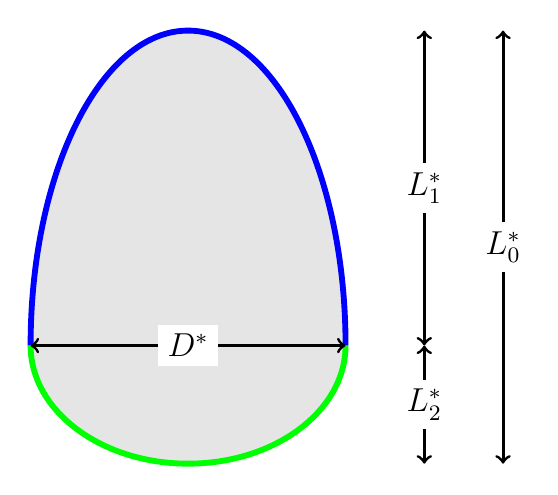
\begin{tikzpicture}
				\filldraw[blue][fill=gray!20!white,line width=0.742mm] (2,0) arc
				[
				start angle=0,
				end angle=180,
				x radius=2cm,
				y radius =4cm
				] ;
				\filldraw[green][fill=gray!20!white,line width=0.742mm] (2,0) arc
				[
				start angle=0,
				end angle=-180,
				x radius=2cm,
				y radius =1.5cm
				] ;
				\coordinate []  (A) at (-2,0)  ;
				\coordinate []  (B) at (2,0) ;
				\coordinate []  (A1) at (3,4)  ;
				\coordinate []  (B1) at (3,-1.5) ;		
				\coordinate []  (A2) at (4,4)  ;
				\coordinate []  (B2) at (4,-1.5) ;		
				\coordinate []  (equator) at (3,0) ;
				\coordinate []  (equator2) at (4,0) ;
				\path[<->] (A) edge[line width=0.371mm] node[ fill=white, anchor=center, pos=0.5,font=\bfseries] {\large $D^*$} (B);
				\path[<->] (equator) edge[line width=0.371mm] node[ fill=white, anchor=center, pos=0.5,font=\bfseries] {\large $L_1^*$} (A1);
				\path[<->] (equator) edge[line width=0.371mm] node[ fill=white, anchor=center, pos=0.5,font=\bfseries] {\large $L_2^*$} (B1);
				\path[<->] (A2) edge[line width=0.371mm] node[ fill=white, anchor=center, pos=0.5,font=\bfseries] {\large $L_0^*$} (B2);
			\end{tikzpicture}
		}
	\end{center}
	\caption{Layout of a constitutive chimera, in profile view. The view represents a vertical cross-section of a shape that is radially symmetrical about the vertical axis. The upper semi-spheroid, with diameter $D^*$ and height $L_1^*$, is shown in blue. The lower semi-spheroid, with diameter $D^*$ and height $L^*_2$, is shown in green. } \label{fig:chimera1}
\end{figure}
\noindent
Figure \ref{fig:chimera1} is a schematic showing the basic geometry of a constitutive chimera.
A constitutive chimera is parameterized by:
\begin{itemize}
	\item $D^*$, the shared diameter of its upper and lower semi-spheroids;
	\item $L_1^*$, the height of its upper semi-spheroid;
	\item $L_2^*$, the height of its  lower semi-spheroid; 
	\item $L_0^* \equiv L_1^* + L_2^*$, the total height of the chimera;
	\item $\alpha \equiv \frac{L_0^*}{D^*}$, an aspect ratio parameter; and,
	\item $\eta \equiv \frac{L_2^*}{L_0^*}$, the fractional height of the lower semi-spheroid.
\end{itemize}
We refer to the junction between the upper and lower semi-spheroids (indicated by $D^*$ in Figure \ref{fig:chimera1}) as the ``equator''.
$\eta$ is the height of the equator, as a fraction of embryo length (\textit{e.g.}, $\eta = 0.5$ implies top-bottom symmetry, $\eta = 0.1$ implies a chimera with a long pointy top and a short, blunt bottom, \etc).
The asterisks imply dimensional quantities.

From the formula for the volume of an spheroid, applied to each semi-spheroid and summed, the total volume of a constitutive chimera is
\begin{equation}\label{vol1}
	V^* = \frac{4 \pi}{3} \left({\frac{D^*}{2}}\right)^2 \left(\frac{L_1^*+L_2^*}{2}\right) = \frac{\pi}{6} {D^*}^2 L_0^*
\end{equation} 
Equation \ref{vol1} shows that the volume is a function of diameter and total length, $L_0^*$, regardless of how that length is allocated to the upper or lower semi-spheroids (that is, the volume is independent of $\eta$).
The volume can also be expressed in terms of the aspect ratio,
\begin{equation}\label{vol2}
	V^* = \frac{\pi}{6} \alpha {D^*}^3
\end{equation} 
From a morphological perspective, this implies that an embryo of fixed diameter $D^*$ and aspect ratio $\alpha$ can develop into a constitutive chimera with the equator at any fractional height, without a change in tissue volume. 

\subsection{Embryos as composites of constitutive chimeras}

\begin{figure}[t] 
	\begin{center}
		\resizebox{6.5cm}{!}{
			
			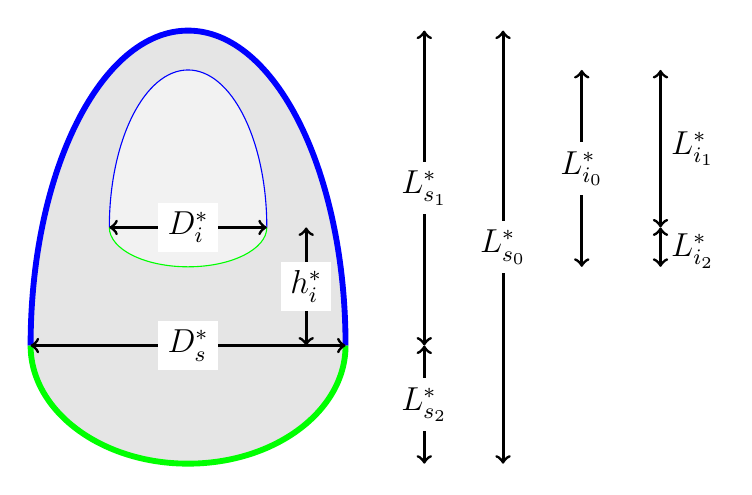
\begin{tikzpicture}
				% Outer (surface) chimera
				\filldraw[blue][fill=gray!20!white,line width=0.742mm] (2,0) arc
				[
				start angle=0,
				end angle=180,
				x radius=2cm,
				y radius =4cm
				] ;
				\filldraw[green][fill=gray!20!white,line width=0.742mm] (2,0) arc
				[
				start angle=0,
				end angle=-180,
				x radius=2cm,
				y radius =1.5cm
				] ;
				\coordinate []  (A) at (-2,0)  ;
				\coordinate []  (B) at (2,0) ;
				\coordinate []  (A1) at (3,4)  ;
				\coordinate []  (B1) at (3,-1.5) ;		
				\coordinate []  (A2) at (4,4)  ;
				\coordinate []  (B2) at (4,-1.5) ;		
				\coordinate []  (equator) at (3,0) ;
				\path[<->] (A) edge[line width=0.371mm] node[ fill=white, anchor=center, pos=0.5,font=\bfseries] {\large $D_s^*$} (B);
				\path[<->] (equator) edge[line width=0.371mm] node[ fill=white, anchor=center, pos=0.5,font=\bfseries] {\large $L_{s_1}^*$} (A1);
				\path[<->] (equator) edge[line width=0.371mm] node[ fill=white, anchor=center, pos=0.5,font=\bfseries] {\large $L_{s_2}^*$} (B1);
				\path[<->] (A2) edge[line width=0.371mm] node[ fill=white, anchor=center, pos=0.5,font=\bfseries] {\large $L_{s_0}^*$} (B2);
				\filldraw[blue][fill=gray!10!white] (1,1.5) arc
				% Inner chimera
				[
				start angle=0,
				end angle=180,
				x radius=1cm,
				y radius =2cm
				] ;
				\draw[green][fill=gray!10!white] (1,1.5) arc
				[
				start angle=0,
				end angle=-180,
				x radius=1cm,
				y radius = 0.5cm
				] ;
				\coordinate []  (A3) at (-1,1.5)  ;
				\coordinate []  (B3) at (1,1.5) ;
				\coordinate []  (A4) at (6,3.5)  ;
				\coordinate []  (B4) at (6,1) ;		
				\coordinate []  (A5) at (5,3.5)  ;
				\coordinate []  (B5) at (5,1) ;		
				\coordinate []  (equator2) at (6,1.5) ;
				\coordinate []  (h0) at (1.5,0) ;
				\coordinate []  (h1) at (1.5,1.5) ;
				\path[<->] (A3) edge[line width=0.371mm] node[ fill=white, anchor=center, pos=0.5,font=\bfseries] {\large $D_i^*$} (B3);
				\path[<->] (equator2) edge[line width=0.371mm] node[anchor=west, pos=0.5,font=\bfseries] {\large $L_{i_1}^*$} (A4);
				\path[<->] (equator2) edge[line width=0.371mm] node[anchor=west, pos=0.6,font=\bfseries] {\large $L_{i_2}^*$} (B4);
				\path[<->] (A5) edge[line width=0.371mm] node[ fill=white, anchor=center, pos=0.5,font=\bfseries] {\large $L_{i_0}^*$} (B5);
				\path[<->] (h0) edge[line width=0.371mm] node[ fill=white, anchor=center, pos=0.5,font=\bfseries] {\large $h_i^*$} (h1);
			\end{tikzpicture}
		}
	\end{center}
	\caption{Layout of a composite chimera, in profile view, with a constitutive chimera representing the exterior surface (parameterized by $D_s^*$, $L^*_{s_0}$, \etc) and a nested constitutive chimera representing an inclusion (parameterized by $D_i^*$, $L^*_{i_0}$, \etc). 
	$h_i^*$ is the height by which the equator of the inclusion chimera is elevated relative to the equator of the surface chimera (which may be negative). 
	%The schematic shows the inclusion chimera being co-axial with the surface chimera. 
	%In the numerical implementation, inclusions may be offset horizontally, as long as no chimera surfaces intersect.
	} \label{fig:chimera2}
\end{figure}
\noindent
Figure \ref{fig:chimera2} is a schematic showing the geometry of a composite chimera, comprising an external constitutive chimera, representing the surface of embryo tissue in contact with the fluid medium, and an internal constitutive chimera representing an inclusion such as lipid, seawater or calcium carbonate.
In the numerical model implementation, an embryo can be constructed with multiple inclusions, e.g. a ``light'' inclusion containing lipids and a ``heavy'' inclusion containing calcium carbonate.
However, to simplify calculations, the numerical model assumes there are no intersections between constitutive chimeras.
That is, \textbf{inclusion chimeras must be entirely inside the surface chimera, and entirely inside or entirely outside of other inclusion chimeras}.

In Figure \ref{fig:chimera2}, $h_i^*$ is the height of the equator of the inclusion, relative to the equator of the surface. 
This parameter is most usefully expressed as the ratio, 
\begin{equation}\label{phi_eq}
	\xi = \frac{h_i^*}{L_{s_0}^*}
\end{equation}
This form anticipates the nondimensionalization below, and its range is constrained such that $-1 < \xi < 1$.

A composite chimera with one inclusion is characterized by three volumes:
\begin{itemize}
	\item $V_s^* = \frac{\pi}{6} \alpha_s {D_s^*}^3$ is the volume enclosed by the outer surface of the composite chimera, with diameter $D_s^*$ and aspect ratio $\alpha_s^*$;
	\item $V_i^* = \frac{\pi}{6} \alpha_i {D_i^*}^3$ is the volume enclosed by the inclusion constitutive chimera, with diameter $D_i^*$ and aspect ratio $\alpha_i^*$; and,
	\item $V_t^* = V_s^* - V_i^*$, the volume of tissue, which is enclosed by the outer surface but outside the inclusion. 
\end{itemize}
We define a volume parameter, $\beta$, quantifying the factor by which total embryo volume is increased relative to tissue volume by an inclusion,
\begin{equation}\label{vol3}
	\beta = \frac{V_s^*}{V_t^*} = 1 + \frac{V_i^*}{V_t^*}.
\end{equation}
In Equation \ref{vol3}, $\beta = 1$ represents an embryo with no inclusion, $\beta = 1.5$ represents an embryo with an inclusion with volume equal to 50\% of the tissue volume, and so on.

If there are multiple inclusions, we distinguish between \textit{exposed} and \textit{contained} inclusions. 
Exposed inclusions are in contact with tissue; therefore, they displace tissue and increase volume within the embryo surface.  
If there are multiple exposed inclusions, then 
\begin{equation}\label{eqn:expincl}
	V_i^* = \sum_{j \in E} V^*_{i_j},
\end{equation}
in  Equation \ref{vol3}, where $E$ is the set of exposed inclusions.
Contained inclusions lie entirely within another inclusion; these do not displace tissue and so do not increase embryo volume (though they do affect calculations of gravity forces, centers of mass, \etc).


If we assume that the embryo increases in size isometrically (that is, for a fixed aspect ratio $\alpha_s$), the change in diameter to maintain a constant tissue volume when an inclusion is added is
\begin{equation}\label{vol4}
	V_s^*  = \frac{\pi}{6} \alpha_s {D_s^*}^3 = \beta V_t^* = \frac{\pi}{6} \alpha_s \beta {D_t^*}^3,
\end{equation} 
from which 
\begin{equation}\label{vol5}
	D_s^* = \sqrt[\uproot{5}3]{\beta} D_t^*.
\end{equation}

%\begin{equation}\label{equivsphere}
%	V_{sph}^* = \frac{\pi}{6} {D_{sph}^*}^3
%\end{equation} 

\subsection{Nondimensionalization: Length scale}
To gain clarity about the distinct roles of \textit{embryo size} and \textit{embryo shape} in swimming performance, we begin by choosing a length scale, $\l$, such that the tissue volume, $\Vts$, has a nondimensionalized value 
\begin{eqnarray}\label{equvol0}
	\Vt \equiv 1
\end{eqnarray} 
Using a nondimensionalization based on a length scale $\l$,
\begin{eqnarray}\label{equvol1}
	\Dt \equiv \frac{\Dts}{\l}
\end{eqnarray} 
we can define $\l$ with 
\begin{eqnarray}\label{equvol2}
	\Vt = \frac{\pi}{6} \alpha_s {\Dt}^3 = \frac{\pi}{6} \alpha_s \left(\frac{\Dts}{\l}\right)^3 = 1,
\end{eqnarray} 
which simplifies to
\begin{eqnarray}\label{equvol3}
	\l \equiv \sqrt[\uproot{5}3]{\frac{\pi \alpha_s}{6}} \Dts
\end{eqnarray} 
It is convenient to define an ``equivalent'' sphere of volume equal to $V_t^*$,
\begin{eqnarray}\label{equivsphere}
	\Vss \equiv \Vts = \frac{\pi}{6} {\Dss}^3,
\end{eqnarray} 
where the equivalent sphere diameter $\Dss$ is
\begin{eqnarray}\label{equvol4}
	\Dss = \sqrt[\uproot{5}3]{\frac{6 \Vts}{\pi}} = \sqrt[\uproot{5}3]{\alpha_s} \Dts .
\end{eqnarray} 
Note that $\l$ can also be expressed as
\begin{eqnarray}\label{equvol3a}
	\l \equiv \sqrt[\uproot{5}3]{\frac{\pi}{6}} \Dss = \sqrt[\uproot{5}3]{\Vts}
\end{eqnarray} 
Adopting these values, the nondimensional forms are
\begin{eqnarray}\label{equvol5}
	\Dt = \sqrt[\uproot{5}3]{\frac{6}{\pi \alpha_s}} \non, \\
	\Ds = \sqrt[\uproot{5}3]{\frac{6}{\pi}}
\end{eqnarray}
Equations \ref{equvol3} (along with \ref{equvol3a}) and \ref{equvol5} are now the basis of a nondimensionalization in which tissue volume is factored out of the rescaled equations.


\section{Nondimensionalized Stokes Equations}\label{NDStokesSect}
Most embryos of marine invertebrates are small enough and move slowly enough to be characterized by a very small to moderately small Reynolds Number, $Re$. 
Flows with $Re = 0$ (\textit{i.e.}, neglecting inertial effects entirely) are described by the Stokes equations, which are linear and are much easier to solve than the Navier-Stokes equations describing higher $Re$ flows.
Though the formal requirement justifying the Stokes equations is $Re \ll 1$, in practice the errors associated with using Stokes equations as approximations for flows with $Re \approx 1$ are typically small.
Here, we assume embryo swimming is characterized by the Stokes equations, accepting the small potential errors associated with inertial effects for the largest and fastest embryos to enable efficient solution techniques.

The dimensional form of the Stokes equations can be written as
\begin{eqnarray}\label{Stokes1}
	0 = \mu^* \left( \frac{\p^2 u^*}{\p {x^*}^2}+\frac{\p^2 u^*}{\p {y^*}^2}+\frac{\p^2 u^*}{\p {z^*}^2} \right) - \frac{\p p^*}{\p {x^*}} + f_x^*, \non \\
	0 = \mu^* \left( \frac{\p^2 v^*}{\p {x^*}^2}+\frac{\p^2 v^*}{\p {y^*}^2}+\frac{\p^2 v^*}{\p {z^*}^2} \right) - \frac{\p p^*}{\p {y^*}} + f_y^*, \non \\
	0 = \mu^* \left( \frac{\p^2 w^*}{\p {x^*}^2}+\frac{\p^2 w^*}{\p {y^*}^2}+\frac{\p^2 w^*}{\p {z^*}^2} \right) - \frac{\p p^*}{\p {z^*}} + f_z^*, \non \\
	0 =  \frac{\p u^*}{\p {x^*}}+\frac{\p v^*}{\p {y^*}}+\frac{\p w^*}{\p {z^*}} 
\end{eqnarray}
In Equations \ref{Stokes1}, $f$ terms denote body forces, with units $\mathrm{\frac{N}{m^3}}$. $p$ is pressure, with units $\mathrm{\frac{N}{m^2}}$.
The first three equations enforce conservation of momentum in the $x$, $y$ and $z$ directions, in the $Re \rightarrow 0$ limit.
The last equation enforces incompressibility.

To nondimensionalize, we define nondimensional parameters $x$, $u$, $p$ and $f_q, q \in x, y, z$:
%,  and $p$ in terms of the characteristic length, $l$, a characteristic body force $$ timescale
\begin{itemize}
	\item We nondimensionalize position and other length quantities by normalizing with $l$:
	\begin{eqnarray*}
		x \equiv \frac{x^*}{\mathit{l}} , \\
		x^* = \mathit{l} x 
	\end{eqnarray*} 
	\item We nondimensionalize velocity by normalizing with $l$ and with a timescale, $\tau^*$, that will be determined below:
	\begin{eqnarray*}
		u \equiv \frac{\tau^*}{\mathit{l}} u^* , \\
		u^* = \frac{\mathit{l}}{\tau^*} u 
	\end{eqnarray*} 
	\item We nondimensionalize body force by normalizing with a characteristic buoyancy force,
	\begin{equation}\label{charforce}
		\hat{f^*} = \Delta \rho ~ g
	\end{equation}
	where $\Delta \rho$ is a ``typical'' density difference between the fluid medium and the embryo. 
	Then, for $q \in x, y, z$:
	\begin{eqnarray*}
		f_q \equiv \frac{f_q^*}{\hat{f^*}}  = \frac{f_q^*}{\Delta \rho^* ~ g} , \\
		f_q^* = \hat{f^*} f_q = \Delta \rho^* ~ g ~ f_q
		%f_q \equiv \frac{\l ~ \tau^*}{\mu^*} f_q^* , \\
		%f_q^* = \frac{\mu^*}{\l ~ \tau^*} f_q 
	\end{eqnarray*} 
	\item Similarly, we nondimensionalize pressure as
	\begin{eqnarray*}
		p \equiv  \frac{ p^*}{\Delta \rho^* ~ g ~ l} , \\
		p^* = \Delta \rho^* ~ g ~ l ~ p  
		%p \equiv \frac{\tau^*}{\mu^*} p^*
		%p^* = \frac{\mu^*}{\tau^*} p, \\
	\end{eqnarray*} 
\end{itemize}
With these nondimensionalizations, the choice 
\begin{equation}\label{tau_def}
	\tau^* = \frac{\mu^*}{\Delta \rho^* ~ g ~ l}
\end{equation}
leads to the nodimensionalized Stokes equations,
\begin{eqnarray}\label{Stokes2}
	0 = \left( \frac{\p^2 u}{\p x^2}+\frac{\p^2 u}{\p y^2}+\frac{\p^2 u}{\p z^2} \right) - \frac{\p p}{\p x} + f_x \non \\
	0 = \left( \frac{\p^2 v}{\p x^2}+\frac{\p^2 v}{\p y^2}+\frac{\p^2 v}{\p z^2} \right) - \frac{\p p}{\p y} + f_y \non \\
	0 = \left( \frac{\p^2 w}{\p x^2}+\frac{\p^2 w}{\p y^2}+\frac{\p^2 w}{\p z^2} \right) - \frac{\p p}{\p z} + f_z , \non \\
	0 =  \frac{\p u}{\p {x}}+\frac{\p v}{\p {y}}+\frac{\p w}{\p {z}}
\end{eqnarray}
In this form of the Stokes Equations. space and time are rescaled such that there are no free parameters -- the primary effects of embryo size, and of the viscosity and density of the fluid medium, are all factored out.  

\subsection{The nondimensionalization timescale, in context}
It is worth a brief consideration of interpretations of $\tau$ as defined in Equation \ref{tau_def}.
Two timescales suggest themselves as being intrinsically relevant to the physics of embryo swimming:
\begin{itemize}
	\item the timescale over which an embryo sinks a distance equal to its own size; and,
	\item the timescale over which an embryo reorients to approach its stable orientation from an initial angular displacement.
\end{itemize}
We can get a sense for the magnitudes of these timescales, without introducing unnecessary parameters, by considering their values for the equivalent sphere.

\subsection{Sinking movement of a sphere}\label{SinkSect}
A sphere of diameter $D_{sph}^*$ sinking in Stokes flow falls at speed
 \begin{equation}\label{sink1}
 	u_{sink}^* = \frac{1}{18} ~ \frac{\Delta \rho^* ~ g}{\mu^*}  ~ {D_{sph}^*}^2,
 \end{equation}
where $\Delta \rho^*$ is the density difference between the sphere and the surrounding fluid.
Defining a timescale $\tau_{sink}$ as the time needed for the sphere to sink a distance equal to the length scale, $l$,
\begin{equation}\label{sink2}
	\tau^*_{sink} = \frac{l}{u_{sink}^*} = 18 \sqrt[\uproot{5}3]{\frac{\pi^2}{36}} ~ \frac{\mu^*}{\Delta \rho^* ~ g ~ l} 
	              = 11.69 ~ \tau^*
\end{equation}
Equation \ref{sink2} shows that the sinking timescale scales in the same way as the timescale inferred in Equation \ref{tau_def} from the nondimensionalization of the Stokes equations, and is larger by an order of magnitude (that is, by a constant factor of 11.69).

\subsection{Rotational movement of a sphere}\label{RotSect}
The rotation rate of a sphere of diameter $D_{sph}^*$ in a fluid of viscosity $\mu^*$ is 
\begin{equation}\label{rot1}
	\omega^* = \frac{T^*}{\pi \mu^* {D_{sph}^*}^3} = \frac{T^*}{6 \mu^* V_{sph}^*},	
\end{equation}
where $T^*$ is the imposed torque (i.e., the imposed moment)\footnote{Ovseensko Y.G. 1969, Refined formulas for the resistance torque of an ellipsoid of revolution and a circular disk rotating in an infinite incompressible viscous fluid. JFM:4(2) pp 100-102.}.

We can define a rotation timescale, $\tau^*_{rot}$, as the inverse of this rate,
\begin{equation}\label{tau1}
	\tau^*_{rot} \equiv {\omega^*}^{-1} = \frac{\pi \mu^* {D_{sph}^*}^3}{T^*} = \frac{6 \mu^* V_{sph}^*}{T^*}
\end{equation}

For the timescale $\tau^*_{rot}$ to reflect the fundamental effects of size on chimera swimming, we can choose a value of $T^*$ that emerges from the equivalent sphere.
$T^*$ is the product of a buoyancy force, $F^*$, and a moment arm $A^*$.
If $F^*$ and $A^*$ are of approximately the same magnitudes as buoyancy forces and moment arms in relevant embryo morphologies, $T^*$ will also be characteristic of buoyancy-driven torque for these morphologies.

As an order-of-magnitude estimate of the moment arm, we can consider a sphere divided along a vertical plane into two hemispheres, one of which differs in density from the surrounding fluid. Using the distance between the center of an equivalent sphere and the centroid of its hemisphere as a moment arm,
\begin{equation}\label{arm}
	A^* = \frac{3}{16} D_{sph}^*
\end{equation}
The buoyancy force is the product of the density difference and the hemisphere volume,
%A density difference, $\Delta \rho^*$, that is likely to be characteristic of many swimming embryo scenarios is indicated by the nominal densities of tissue, $\rho_{tissue} = 1070 ~ \mathrm{\frac{kg}{m^3}}$, and of lipid, $\rho_{lipid} = 900 ~ \mathrm{\frac{kg}{m^3}}$, in comparison to seawater, $\rho_{seawater} = 1030 ~ \mathrm{\frac{kg}{m^3}}$.
%Expressing the density difference in terms of $\rho_{seawater}$,
%\begin{equation}\label{dens}
%	\Delta \rho^* = \gamma ~ \rho_{med},
%	%\Delta \rho^* = \rho_{tissue} - \rho_{lipid}
%\end{equation}
%where the coefficient $\gamma$ is of $\mathcal{O}(10^{-1})$ so that $\Delta \rho^* \approx 10^2$.
%%Taking $\rho_{tissue} = 1070 ~ \mathrm{\frac{kg}{m^3}}$ and $\rho_{lipid} = 900 ~ \mathrm{\frac{kg}{m^3}}$ as nominal values gives a value for the characteristic density difference driving embryo rotation as
%%\begin{equation}\label{dens2}
%%	\Delta \rho^* = 130 ~ \mathrm{\frac{kg}{m^3}}
%%\end{equation}
%
%Using the volume from the equivalent hemisphere, 
\begin{equation}\label{charF}
	F_{sph}^* = \frac{\Delta \rho^* ~ g ~ V_{sph}^*}{2}.  %= \frac{\pi}{6} ~ \rho_{med}^* ~ g ~ {D_{sph}^*}^3,
\end{equation} 
Combining these estimates,
\begin{equation}\label{charT}
	T^* \equiv F^* ~ A^* = \frac{3}{32} ~ \Delta \rho^* ~ g ~ D_{sph}^* V_{sph}^* 
	% = \frac{3 \pi}{192} ~ \Delta \rho^* ~ g ~ {D_{sph}^*}^4
\end{equation}
is a characteristic buoyancy-driven torque for many relevant embryo morphologies.
% 
%\begin{equation}\label{charT}
%	T^* \equiv F^* ~ A^* = \frac{\Delta \rho^* ~ g ~ V_{sph}^*}{2} ~ \frac{3 ~ D_{sph}^*}{16} =  %D_{sph}^* F_{sph}^* = \frac{\pi}{6} ~ \rho_{med}^* ~ g ~ {D_{sph}^*}^4 =  \rho_{med}^* ~ g ~ D_{sph}^* V_{sph}^*,
%\end{equation} 
%
%\begin{eqnarray}\label{charT2}
%	T^* & = & \frac{3}{32} ~ \Delta \rho^* ~ g D_{sph}^* V_{sph}^* \non \\
%	    & = & \frac{3}{32} ~ \Delta \rho^* ~ g D_{sph}^* \frac{\pi}{6} {D_{sph}^*}^3 \non \\
%	    & = & \frac{3 \pi}{192} ~ \Delta \rho^* ~ g ~ {D_{sph}^*}^4
%	%D_{sph}^* F_{sph}^* = \frac{\pi}{6} ~ \rho_{med}^* ~ g ~ {D_{sph}^*}^4 =  \rho_{med}^* ~ g ~ D_{sph}^* V_{sph}^*,
%\end{eqnarray} 

Substituting this value into Equation \ref{tau1}, substituting with \ref{equvol4} and simplifying gives
\begin{equation}\label{tau2}
	\tau^*_{rot} = \frac{64 ~ \mu^*}{\Delta \rho^* ~ g ~ D_{sph}} 
	=  64\sqrt[\uproot{5}3]{\frac{\pi}{6}} ~ \tau^*
%=  64\sqrt[\uproot{5}3]{\frac{\pi}{6}} \frac{\mu^*}{\Delta \rho^* ~ g ~ l}
\end{equation}
Equation \ref{tau2} shows that the rotation timescale scales in the same way as the timescale inferred in Equation \ref{tau_def} from the nondimensionalization of the Stokes equations, and is larger by about two orders of magnitude (that is, by a constant factor of 51.58).

The consistency in scaling of Equations \ref{sink2} and \ref{tau2} with Equation \ref{tau_def} shows that very similar nondimensionalizations (differing only by constant factors) are obtained by these three distinct approaches to determining relevant timescales for the embryo swimming problem.
The relative magnitudes, in which sinking and rotation timescales are 1-2 orders larger than the nominal timescale $\tau^*$, suggests that simulations of embryo swimming must have minimum durations of roughly 3 orders of magnitude larger than $\tau$ to reflect the effects of environment on orientation and water column position.


\section{Parameterization of the non-dimensional embryo swimming problem}\label{NDparsSect}
This section summarizes the procedure to convert dimensional parameters from a scenario of embryo swimming into their nondimensional parameter analogs, and to reconvert nondimensional results into their corresponding dimensional quantities.
The expectation is that results from directly simulating a dimensional scenario are identical to results from converting that scenario to its nondimensional counterpart, running the simulation, and re-dimensionalizing the results.
That being established, each nondimensional result is applicable to a wide range of dimensional scenarios. This reduction in parameter space facilitates an overall analysis of embryo swimming functional morphology.

The basic strategy is to derive the \textit{shape parameters}, 
\begin{eqnarray}\label{shapars}
	\alpha_s, \eta_s, \alpha_{i}, \eta_{i}, \beta, \xi
\end{eqnarray}
from the experimentally observed embryo dimensions.
These shape parameters, together with three \textit{scale parameters} -- tissue volume $\Vts$ and the fluid medium viscosity $\mu^*$ and density $\rho_{med}^*$ -- are then sufficient to reconstruct:
\begin{itemize}
	\item the original observed geometry and swimming scenario;
	\item the corresponding nondimensional geometry and swimming scenario;
	\item any other geometrically and dynamically similar geometry and swimming scenario.
\end{itemize}
%Because the nondimensional geometry corresponds to a spectrum of dynamically similar physical geometries, swimming performance measured on the nondimensional geometry can be used to infer the performance of the entire spectrum of dynamically similar embryos.
The shape parameters summarize the geometry of an early stage embryo with tissue volume factored out, opening the possibility of separately delineating the effects of embryo size and shape.
Essentially, this parameterization frames the questions,
\begin{quotation}
	\textbf{What are the inherent constraints on swimming performance for embryos of different sizes?}
\end{quotation}
\begin{quotation}
	\textbf{Given a fixed amount of tissue, what are the costs and benefits of forming that tissue into embryos of different shapes?}
\end{quotation}

\subsection{Dimensional to nondimensional conversion}
A typical dimensional embryo swimming scenario is prescribed by:
\begin{itemize}
	\item Geometrical parameters of the outer surface: $D^*_s$, $L^*_{s_0}$, $L^*_{s_1}$, $L^*_{s_2}$; 
	\item Geometrical parameters of the inclusion(s): $D^*_{i}$, $L^*_{i_0}$, $L^*_{i_1}$, $L^*_{i_2}$, $h^*_i$; 
	\item Densities of the tissue and inclusion(s): $\rho^*_t$, $\rho^*_{i}$; 
	\item Ciliary velocity: $v^*_{cil}$;
	\item Fluid medium viscosity and density: $\rho^*_{med}$, $\mu^*$;
	\item Fluid medium shear, $\frac{\p u^*}{\p z^*}$, $\frac{\p w^*}{\p x^*}$ and $\frac{\p w^*}{\p y^*}$
	\item Simulation end time, $t^*_{end}$;
	\item Initial position, $(x^*, y^*, z^*) = (0,0,0)$; and,
	\item Initial orientation, specified by Euler angles $\phi$, $\theta$ and $\psi$. 
\end{itemize}
Geometrical parameters and ciliary velocity are typically measured on micrographs or microvideos (Fig. \ref{fig:chimera2}).
Densities are often estimated from equilibrium positions in water columns with density gradients (to measure average density) or inferred from known properties of specific materials (seawater, lipids, calcium carbonate, \etc). 
The Euler angles, $\phi$, $\theta$ and $\psi$,  have units of radians, and are not changed in the nondimensionalization.
Relevant ranges for the shears are inferred from \textit{in situ} observations of turbulence or estimates of turbulent intensity in different marine habitats.

From these parameters, the steps to obtain the corresponding nondimensional parameter set are:
\begin{enumerate}
	\item Calculate the volumes:
	\begin{eqnarray}\label{d2ndpars2}
		V_s^* = \frac{\pi}{6} L_{s_0}^* {D_s^*}^2 \non \\
		V_i^* = \frac{\pi}{6} L_{i_0}^* {D_i^*}^2 \non \\
		V_t^* = V_s^* - V_i^* 
	\end{eqnarray}
	\item Calculate the shape parameters: %aspect ratio and equatorial height parameters:
	\begin{eqnarray}\label{d2ndpars1}
		\alpha_s = \frac{L^*_{s_0}}{D^*_s} \non \\
		\eta_s = \frac{L^*_{s_2}}{L^*_{s_0}} \non \\
		\alpha_{i} = \frac{L^*_{i_0}}{D^*_i} \non \\
		\eta_{i} = \frac{L^*_{i_2}}{L^*_{i_0}} \non \\
		\xi = \frac{h_i^*}{L_{s_0}^*} \non \\
		\beta = \frac{V_s^*}{V_t^*}
		%D_t^* = \frac{1}{\sqrt[\uproot{5}3]{\beta}} D_s^*
	\end{eqnarray}
	%\item Calculate the characteristic length, the equivalent sphere diameter and the rotation timescale:
	\item Calculate the characteristic length and timescale:
	\begin{eqnarray}\label{d2ndpars3}
		\l = \sqrt[\uproot{5}3]{V_t^*} \non \\
		%D_{sph}^* = \sqrt[\uproot{5}3]{\frac{6}{\pi} V_t^*} \non \\
		%\l = \sqrt[\uproot{5}3]{\frac{\pi}{6}} D_{sph}^* \non \\
		%\tau^* = \frac{6  \mu^*}{\rho^*_{med} ~ g ~ D_{sph}^*}
		\Delta \rho^* = \gamma \rho_{med}^*, ~ \gamma = 0.1 \non \\
		\tau^* = \frac{\mu^*}{\Delta \rho^* ~ g ~ l}
	\end{eqnarray}
	Here, a ``typical'' density difference equal to $\gamma \rho_{med}^*$ is assumed in determining the timescale, to streamline comparisons of nondimensional swimming performance across variations in embryo density.
	The value $\gamma = 0.1$ reflects the order of magnitude of density differences of embryo tissue, lipid, freshwater etc.
	\item Calculate the nondimensionalized geometrical parameters:
	\begin{eqnarray}\label{d2ndpars4a}
		D_t = \sqrt[\uproot{5}3]{\frac{6}{\pi \alpha_s}} \non \\
		D_s = \sqrt[\uproot{5}3]{\frac{6 \beta}{\pi \alpha_s}} \non \\
		L_{s_0} = \alpha_s D_s \non \\
		L_{s_2} = \eta_s L_{s_0} \non \\
		 L_{s_1} = (1 - \eta_s) L_{s_0} \non \\
		%L_{s_2} = \eta_s L_{s_0}, L_{s_1} = L_{s_0} - L_{s_2} \non \\
		%V_i = \frac{V^*_i}{V^*_t} \non \\
		V_i = \beta - 1 \non \\
		D_i = \sqrt[\uproot{5}3]{\frac{6 (1-\beta)}{\pi \alpha_i}} \non \\
		%D_i = \sqrt[\uproot{5}3]{\frac{6 V_i}{\pi \alpha_i}} \non \\
		L_{i_0} = \alpha_i D_i \non \\
		L_{i_2} = \eta_i L_{i_0} \non \\
		 L_{i_1} = (1 - \eta_i) L_{i_0} \non \\
		h_i = \xi L_{s_0} 
		%h_i = \frac{h^*_i}{D_t^*}
		%L_{i_1} = \frac{L^*_{i_1}}{D_{sph}^*}, L_{i_2} = \frac{L^*_{i_2}}{D_{sph}^*}, D_i = \frac{D^*_i}{D_{sph}^*}, h_i = \frac{h^*_i}{D_{sph}^*}
	\end{eqnarray}
	\item Calculate the nondimensionalized tissue and inclusion densities:
	\begin{eqnarray}\label{d2ndpars5}
		\rho_t = \frac{\rho_t^*}{\Delta \rho^*} \non \\
		\rho_i = \frac{\rho_i^*}{\Delta \rho^*}
	\end{eqnarray}
	\item Calculate the nondimensionalized ciliary velocity, shear and simulation end time:
	\begin{eqnarray}\label{d2ndpars6}
		v_{cil} = \frac{{\tau^*}}{\l}  v^*_{cil} \non \\
		\frac{\p w}{\p x} = \tau^* \frac{\p w^*}{\p x^*} \non \\
		\frac{\p u}{\p z} = \tau^* \frac{\p u^*}{\p z^*} \non \\
		t_{end} = \frac{t^*_{end}}{\tau^*}
	\end{eqnarray}
\end{enumerate}

\newpage 
\subsection{Nondimensional to dimensional conversion}
To relate nondimensional results to real-world scenarios in physical units, the required physical parameters are
\begin{eqnarray}\label{nd2dpars0}
	D^*_s, L^*_{s_1}, L^*_{s_2}, D^*_{i}, L^*_{i_1}, L^*_{i_2}, h^*_i, \rho^*_t, \rho^*_{i}, V^*_{cil}, \rho^*_{med}, \mu^*, \frac{\p u^*}{\p z^*}, \frac{\p w^*}{\p x^*}, t^*_{end}.
\end{eqnarray}
These must be derived from the following sets of parameters:
\begin{itemize}
	\item The three physical \textit{scale parameters},
		\begin{eqnarray}\label{nd2dpars0a}
			V_t^*, \mu^*, \rho^*_{med}	
		\end{eqnarray}
	\item The \textit{shape parameters}, 
		\begin{eqnarray}\label{nd2dpars2}
			\alpha_s, \eta_s, \alpha_{i}, \eta_{i}, \beta, \xi
		\end{eqnarray}
	\item The nondimensional tissue and inclusion densities, and ciliary velocity:
		\begin{eqnarray}\label{nd2dpars1a}
			v_{cil}, \rho_t, \rho_i, \frac{\p w}{\p x}, \frac{\p u}{\p z}, t_{end}
		\end{eqnarray}
	\item The ciliary velocity, shears and simulation end time:
		\begin{eqnarray}\label{nd2dpars1b}
			v_{cil}, \frac{\p w}{\p x}, \frac{\p u}{\p z}, t_{end}
		\end{eqnarray}
	\item The initial Euler angles and position
		\begin{eqnarray}\label{nd2dpars2a}
			\phi, \theta, \psi, x_0, y_0, z_0
		\end{eqnarray}	 	
\end{itemize}
%\begin{eqnarray}\label{nd2dpars1}
%	D_s, L_{s_0}, L_{s_2}, L_{s_1}, V_i, D_i, L_{i_0}, L_{i_2}, L_{i_0}, L_{i_1}, \non \\
%	h_i, v_{cil}, \rho_t, \rho_i, \frac{\p w}{\p x}, \frac{\p u}{\p z}, t_{end}
%\end{eqnarray}
The shape parameters and the initial Euler angles apply equally to both dimensional and nondimensional scenarios.


\begin{enumerate}
	\item From these, calculate tissue and surface volumes, tissue and inclusion densities, the equivalent sphere diameter and the rotation timescale :
\begin{eqnarray}\label{nd2dpars3}
	\Delta \rho^* = \gamma ~ \rho_{med}^*, ~ \gamma = 0.1 \non \\
	\rho^*_t = \Delta \rho^* ~ \rho_t \non \\
	\rho^*_i = \Delta \rho^* ~ \rho_i \non \\
	V_s^* = \beta V_t^* \non \\
	V_i^* = (\beta-1) V_t^* \non \\
	\l = \sqrt[\uproot{5}3]{V_t^*} \non \\
	%D_{sph}^* = \sqrt[\uproot{5}3]{\frac{6}{\pi}} \l \non \\
	%\tau^* = \frac{6 \mu^*}{\rho^*_{med} ~ g ~ D_{sph}^*} \\
	\tau^* = \frac{\mu^*}{\Delta \rho^* ~ g ~ l}
\end{eqnarray}
\item Calculate dimensions of the surface and inclusions in physical units:
\begin{eqnarray}\label{nd2dpars4}
	%D_t^* = \sqrt[\uproot{5}3]{\frac{6}{\pi \alpha_s}} \l \non \\
	D_s^* = \sqrt[\uproot{5}3]{\frac{6 \beta}{\pi \alpha_s}} \l \non \\
	%D_s^* = \sqrt[\uproot{5}3]{\beta} D_t^* \non \\
	D^*_i = \sqrt[\uproot{5}3]{\frac{6 (\beta-1)}{\pi \alpha_i}} \l \non \\
	L^*_{s_0} = \alpha_s D^*_s \non \\
	L^*_{s_2} = \eta_s L^*_{s_0} \non \\
	L^*_{s_1} = (1-\eta_s) L^*_{s_0} \non \\
	L^*_{i_0} = \alpha_i D^*_i \non \\
	L^*_{i_2} = \eta_i L^*_{i_0} \non \\
	L^*_{i_1} = (1-\eta_i) L^*_{i_0} \non \\
	h^*_i = \xi L^*_{s_0}  \non \\
\end{eqnarray}
%\begin{eqnarray}\label{nd2dpars4}
%	D_t^* = \sqrt[\uproot{5}3]{\frac{6 V_t^*}{\pi \alpha_s}} \non \\
%	D_s^* = \sqrt[\uproot{5}3]{\beta} D_t^* \non \\
%	D^*_i = \sqrt[\uproot{5}3]{\frac{6 V_i^*}{\pi \alpha_i}} \non \\
%	L^*_{s_0} = \alpha_s D^*_s \non \\
%	L^*_{s_2} = \eta_s L^*_{s_0} \non \\
%	L^*_{s_1} = (1-\eta_s) L^*_{s_0} \non \\
%	L^*_{i_0} = \alpha_i D^*_i \non \\
%	L^*_{i_2} = \eta_i L^*_{i_0} \non \\
%	L^*_{i_1} = (1-\eta_i) L^*_{i_0} \non \\
%	h^*_i = \xi L^*_{s_0}  \non \\
%\end{eqnarray}
\item Calculate ciliary velocity, shear and simulation time:
\begin{eqnarray}\label{nd2dpars4a}
	v^*_{cil} = \frac{\l}{\tau^*}  v_{cil} \non \\
	\frac{\p w^*}{\p x^*} = \frac{1}{\tau^*} \frac{\p w}{\p x} \non \\
	\frac{\p u^*}{\p z^*} = \frac{1}{\tau^*} \frac{\p u}{\p z} \non \\
	t^*_{end} = \tau^* t_{end}
\end{eqnarray}
	
\end{enumerate}


%\begin{table}[h]
%	\centering
%	\caption{Summary of dimensional-nondimensional transformations for the swimming embryo problem. In the left column, $\sim$ is followed by the SI units of the dimensional parameter. Parameters that have units $\sim 1$ are already nondimensional, and are unchanged in the nondimensionalization. Among dimensional-nondimensional parameter pairs, the dimensional form is labeled with an $^*$. The diameter of the equivalent sphere, $D_{sph}^*$, is given in Equation \ref{equivsphere} . The rotation timescale, $\tau^*$, is given in Equation \ref{tau2} .} \label{tab:d2nd}
%	\vspace{.25cm}
%	\small
%	\rowcolors{2}{gray!10}{white}
%	\begin{tabular}{|I|L|l|}
%		\hline
%		Dimen. param. & Conversion formula \& result & \hspace{1cm} Interpretation \\
%		\hline
%		$\rho_t^* \sim \mathsf{\frac{kg}{m^3}}$ & $\rho_t = \frac{1}{\rho_{med}^*} \rho_t^* $  & Density of tissue \\
%		$V^*_t \sim \mathsf{m^3}$ & $V_t = \frac{1}{{D_{sph}^*}^3} V^*_t $  & Volume of tissue \\
%		$\alpha_s \sim \mathsf{1}$ & $\alpha_s = \frac{L^*_{s_0}}{D^*_s}, ~ L^*_{s_0} = L^*_{s_1} + L^*_{s_2}$ & Aspect ratio of embryo surface \\
%		$\eta_s \sim \mathsf{1}$ & $\eta_s = \frac{L^*_{s_2}}{L^*_{s_0}}$ & Equatorial height of embryo surface \\
%		$\rho_m^* \sim \mathsf{\frac{kg}{m^3}}$ & $\rho_m = \frac{1}{\rho_{med}^*} \rho_m^* $  & Density of embryo material $m$ \\
%		$V^*_{i_m} \sim \mathsf{m^3}$ & $V_{i_m} = \frac{1}{{D_{sph}^*}^3} V^*_{i_m} $  & Volume of inclusion $m$ \\
%		$\alpha_{i_m} \sim \mathsf{1}$ & $\alpha_i = \frac{L^*_{i_0}}{D^*_i}, ~ L^*_{i_0} = L^*_{i_1} + L^*_{i_2}$ & Aspect ratio of inclusion $m$ \\
%		$\eta_{i_m} \sim \mathsf{1}$ & $\eta_i = \frac{L^*_{i_2}}{L^*_{i_0}}$ & Equatorial height of inclusion $m$ \\
%		$h^*_{i_m} \sim \mathsf{m}$ & $h_{i_m} = \frac{1}{{D_{sph}^*}} h^*_{i_m} $  & Vertical position of inclusion $m$ \\
%		$v^*_{cil} \sim \mathsf{\frac{m}{s}}$ & $v_{cil} = \frac{{\tau^*}}{D_{sph}^*}  v^*_{cil}  $  & Ciliary velocity \\
%		%$v^*_{cil} \sim \mathsf{\frac{m}{s}}$ & $v_{cil} = \frac{D_{sph}^*}{{\tau^*}}  v^*_{cil}  = 6 \frac{\mu^*}{{\rho_{med}^* g}}  v^*_{cil} $  & Ciliary velocity \\
%		\hline
%		\vspace{0.1cm}
%		$\frac{\p w^*}{\p x^*} \sim \mathsf{\frac{1}{s}}$ & $\frac{\p w}{\p x} = \tau^* \frac{\p w^*}{\p x^*}  $  & Vertical shear velocity \\
%		\vspace{0.1cm}
%		$\frac{\p u^*}{\p z^*} \sim \mathsf{\frac{1}{s}}$ & $\frac{\p u}{\p z} = \tau^* \frac{\p u^*}{\p z^*}  $  & Horizontal shear velocity \\
%		\vspace{0.1cm}
%		$t^* \sim \mathsf{s}$ & $t =  \frac{t^*}{\tau^*}  $  & Time \\
%		\hline
%	\end{tabular}
%\end{table}
%


















\end{document}